\documentclass[a4paper,10pt]{jsarticle}
\usepackage[left=2cm,right=2cm,top=3cm,bottom=3cm]{geometry}
\usepackage{multicol}
\usepackage{blindtext}
\usepackage{amsmath,amsfonts}
\usepackage{bm}
\usepackage{siunitx}
\usepackage[dvipdfmx]{graphicx}
\usepackage{booktabs}
\usepackage{multirow}
\usepackage{here}
\usepackage{wrapfig}
\usepackage{textcomp}

\setlength{\columnsep}{10mm}
\makeatletter
\newenvironment{tablehere}
{\def\@captype{table}}
{}
\newenvironment{figurehere}
{\def\@captype{figure}}
{}
\makeatother

\begin{document}
\title{{ スペクトル分解能と屈折率の波長依存性について}}
\author{Teduka Yuuki 1522063 
\\
Collaborator:Nakamura Kouta 1522B02, Mizusiri Keigo 1522089 }
\date{Lab date: 18th and 25th April 2023}
\maketitle

\begin{abstract}
  この実験の目的は主に三つある。
  一つ目は、波長分布を既知とする光をスペクトル分解し、スペクトル分解能について考察することである。スペクトル分解能とは、同時に異なる波長または周波数の光や電磁波を区別する能力のことを指す。
  二つ目は、光の屈折率の波長依存性を調べることである。屈折率は透明物質では可視光領域で一般に短波長ほど屈折率が大きくなる。
  三つ目は、白色LEDのスペクトル分布を調べることである。
  これらの目的に基づいて、以下の三つの実験を行った。
  実験1では、波長分布が与えられたNa,Hg,Cdランプの光をスリットに通し、反射型回折格子に反射させ、分散した光をスクリーンで観測することで、スペクトル分解を行った。
  Cdランプについてはスリット幅が1000\textmu mの時と、200\textmu mの時でスペクトルを観測した。その結果、スリット幅を狭めた方が、スペクトル分解能を向上させることがわかった。
  実験2では、ガラス製三角プリズムにCdランプの光を入射させ、最小偏角を測定することで屈折率を求めた。波長は実験1で求めた値を用いて、波長に対する屈折率の波長依存性を調べた。その結果、屈折率は波長が短くなるにつれて大きくなることが確認できた。
  実験3では、白色LEDのスペクトル分布を調べた。白色LEDのスペクトル分布は、一様ではなく、青色と黄色の二つのピークがあることがわかった。
  
\end{abstract}

\begin{multicols}{2}
\section{Introduction}
\subsection{屈折率の波長依存性}
よく知られているように、ある波長$\lambda$の光線が、媒質1から媒質2に斜めに入射する場合、入射角$i$と屈折角$r$の間には以下の関係が成り立つ。

\begin{equation}
  \sin{i}/\sin{r} = n_{21} = constant
\end{equation}

$n_{21}$は、媒質2の媒質1に対する相対屈折率で、特に媒質1が真空の場合は$n_{2}\equiv n_{21}$を絶対屈折率という。
$n_{21}$は、入射角$i$が変化しても変わらないが、波長や媒質の温度が変われば変化する量で、特に波長の変化に対する屈折率の変化を分散(dispersion)という。分散自身をまた波長に依存する量である。屈折率の波長依存性は、透明物質では可視光領域で一般に短波長ほど屈折率が大きくなっている。これを正常分散(normal dispersion)という。
これに対して、強い吸収のある領域では、逆に短波長に向かって、屈折率が減少していくことがある。これを異常分散(anomalous dispersion)という。

\begin{figurehere}
\centering
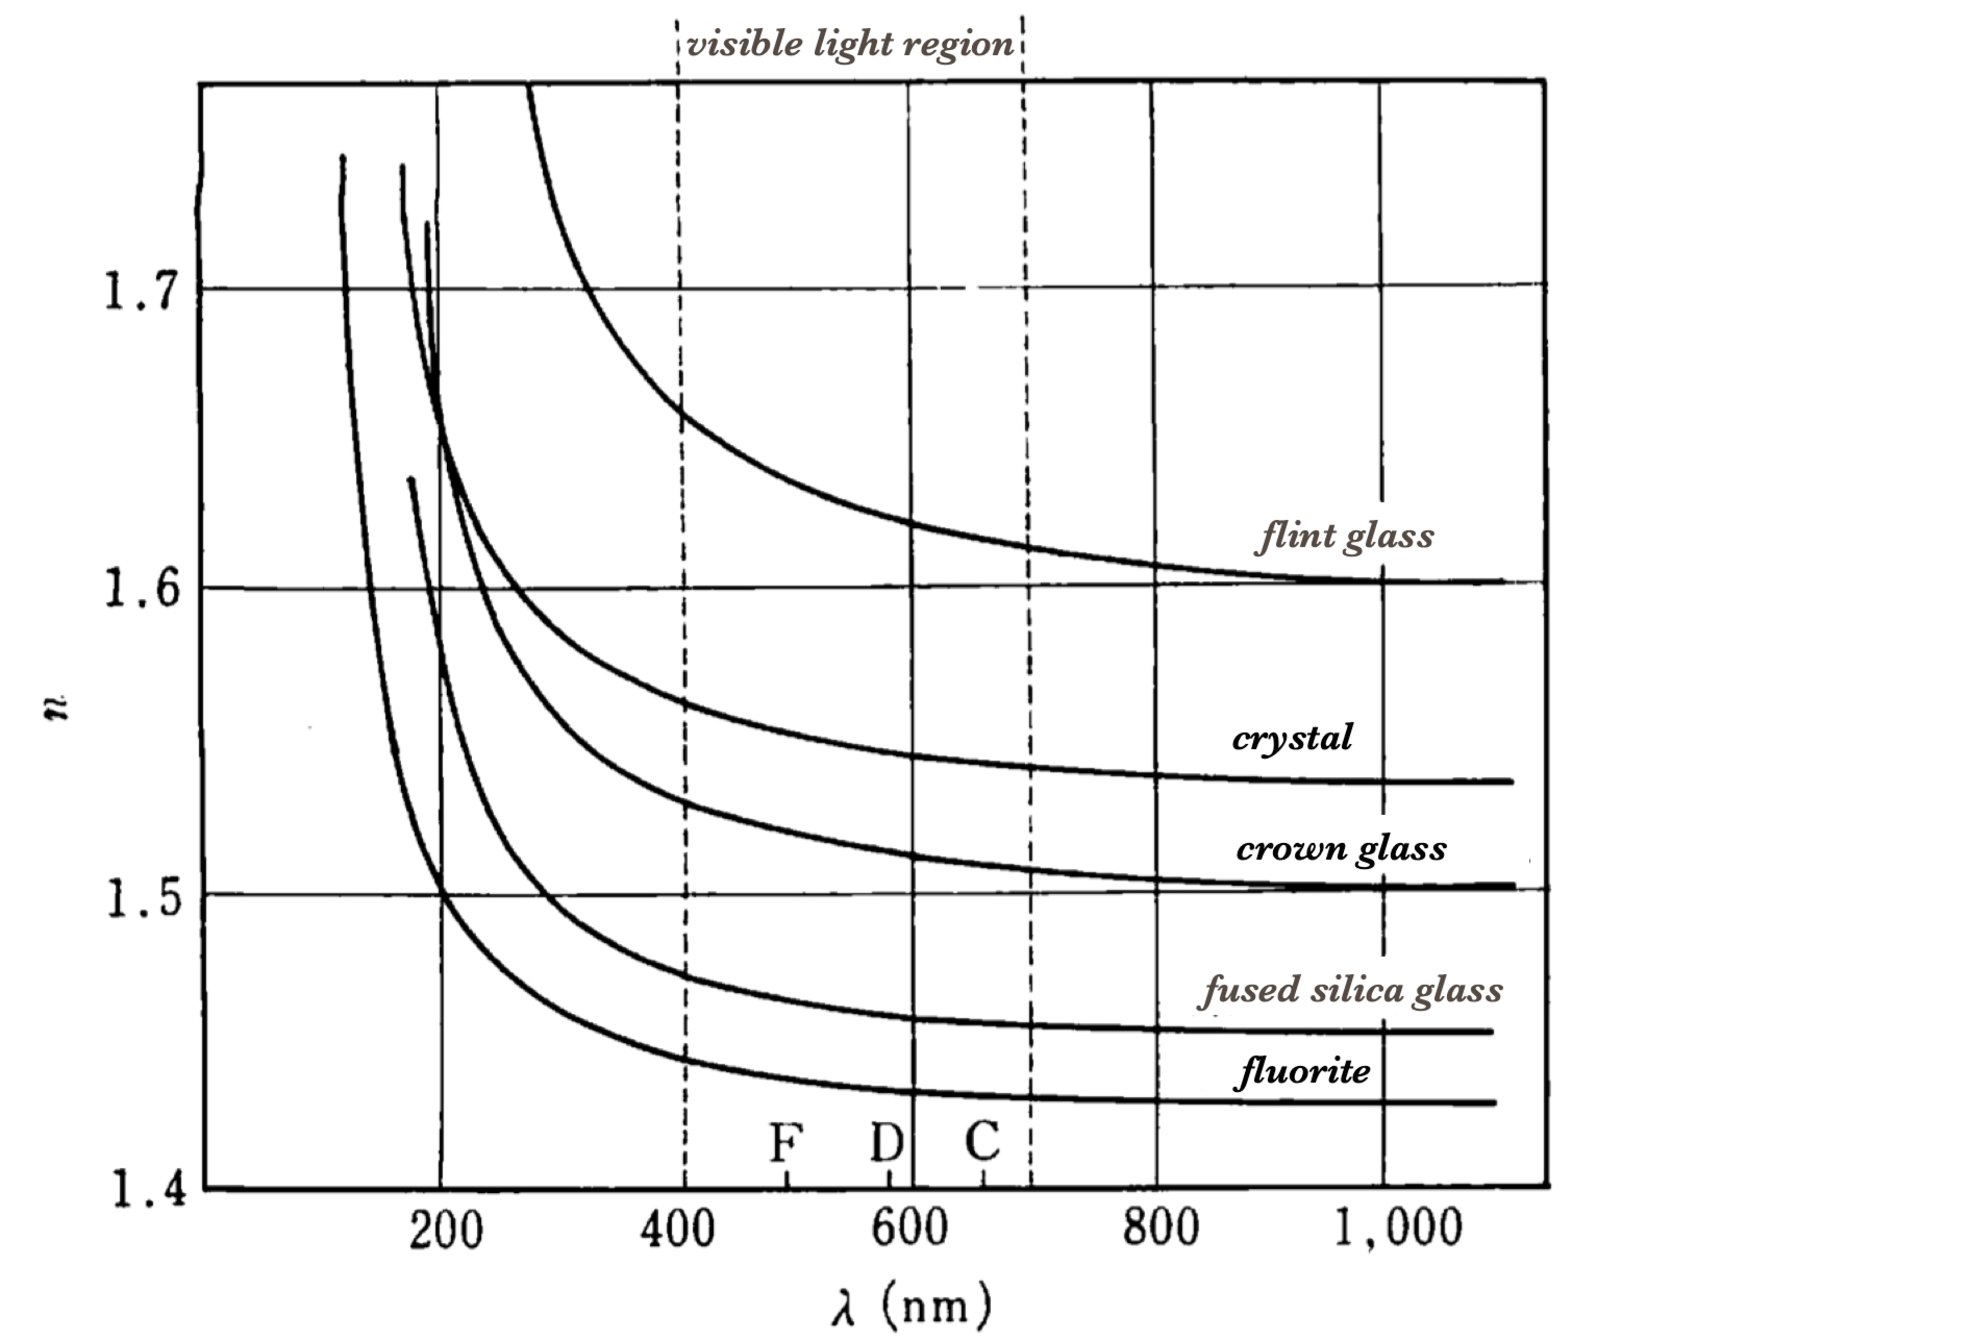
\includegraphics[width=0.55\textwidth]{figs/kusseturitu.pdf}
\caption[]{%
光学材料の屈折率の波長依存性
\footnotemark}
\end{figurehere}
\footnotetext{%
参考: https://annex.jsap.or.jp
}

図1に、よく用いられる光学材料の屈折率の波長依存性を示した。
屈折率の変化は波長に対して直線的ではないが、波長領域を可視光に限れば、ほぼ直線的と見做し得る。
従って、各波長$\lambda$に対する屈折率$n$を求め、$n$-$\lambda$グラフにプロットした場合、直線的になるはずである。実験2-2でこれを確かめた。。
屈折率の絶対測定には、測定したい物質で三角プリズムを作り、一つの斜面にある波長の光線を入射させ、他面から出てくる光線との角、すなわち偏角$\delta$を測定する。$\delta$は入射角によって変わるが、極小値$\delta_{min}$をもつ。プリズムの頂角を$\alpha$とすると、屈折率$n$は、
\begin{equation}
  n =\sin\{(\alpha+\delta_{min})/2\}/\sin(\alpha/2)
\end{equation}
で計算できる。
この式は付録で導出する。
つまり、$\alpha$を既知として、各波長$\lambda$における$\delta_{min}$を測定することで、各波長に対する屈折率を測定できる。
% しかし問題は、$\delta_{min}$をいかに正確に測定できるかということである。
\subsection{反射型回折格子による波長分布の測定}

\begin{figurehere}
\centering
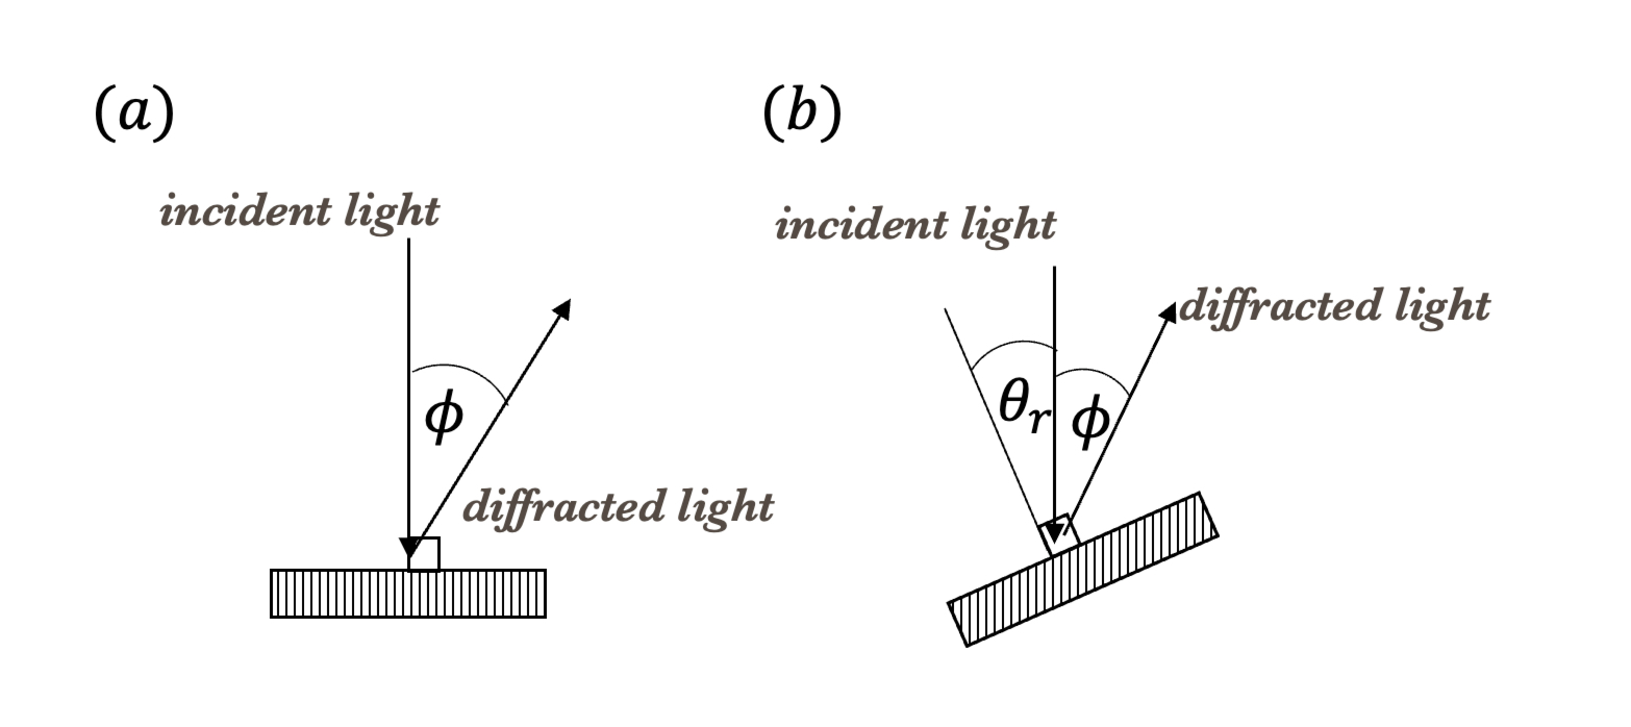
\includegraphics[width=0.55\textwidth]{figs/kaisekikousi.pdf}
\caption{入射光と検出光の経路のなす角を固定した場合の入射角と回析角}
\label{fig:fig1}
\end{figurehere}
反射型回折格子を用いたスペクトル測定は、光の波長を分散するために使用される実験法の一つである。回折格子は、平行な溝が等間隔に彫られた平板であり、入射した光を反射させることで波長ごとに分散する。

この実験法では、まず回折格子を入射光に対して正しく配置し、回折格子上に狭い光束を当てる。回折格子上に入射した光は、溝の間隔によって反射され、スクリーン上に分散して映し出される。スクリーン上に映し出された分散された光を観察することで、入射光の波長分布を測定することができる。

図2のように反射型回折格子に光を入射させた場合を考える。図1-$(a)$のように、入射光と回析光のなす角を$\phi$とし、図1-$(b)$のように回折格子を$\theta_r$だけ回転させた時、検出される回折光の条件は、
\begin{equation}
  d\{\sin(\theta_r+\phi)+\sin\theta_r\} = m\lambda
\end{equation}
で与えられることは分かる。

$m$は回折の次数を表しているので、$d$を既知とし、入射光と回析光のなす角$\phi$を測定することで、波長$\lambda$を求めることができる。

\subsection{白色LEDのスペクトル}
図3から分かるように、一般に使用されている白色LEDはスペクトル分布に偏りがある。
465nmあたりで鋭いピークがあり、560nmあたりでも、緩やかなピークが見られる。
一般に使用されている白色LEDは、青色光を出す青色LEDと黄色光を出す蛍光物質を組み合わせたものであり、
青色と黄色は補色の関係にあるため、青色光と黄色光を混ぜ合わせた光が白色光として見えている。
\\

\begin{figurehere}
 \centering
 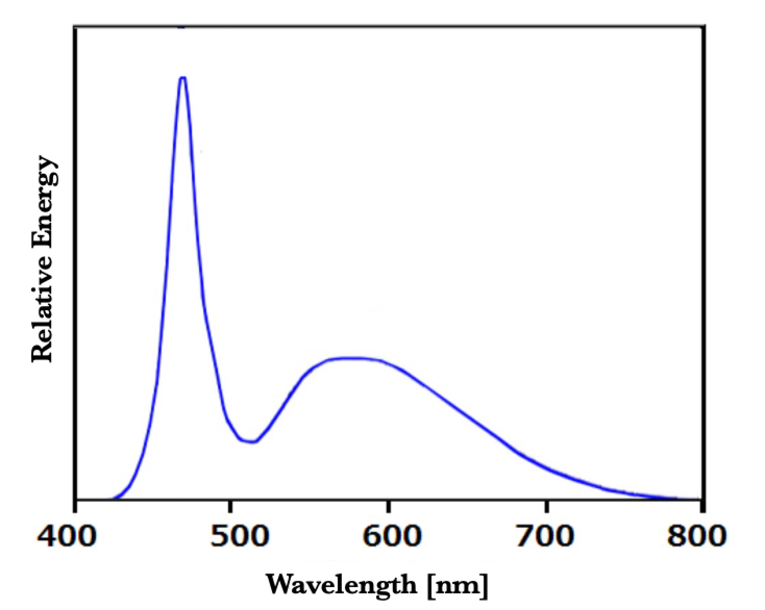
\includegraphics[width=0.5\textwidth]{figs/led_sample.pdf}
 \caption{擬似白色発LEDのスペクトル}
\end{figurehere}




\clearpage
\end{multicols}
\section{Methods}

[実験装置]:

ブレッドボード、波長可変スリット、平凸レンズ、両凸レンズ、ブームプロッカー、スクリーン.

フォトダイオード : 検出素子前に、幅200\textmu mのスリットを付けている。

プリズム : ガラス製のプリズムを用いる。 形状は正三角形であり、頂角は60°である。

反射型回折格子(Thorlabs: GR25-1205) : 刻線数は 1200 lines/mm、 ブレーズ波長 500 nm。

Na, Cd, Hgランプ : ランプの光は安定するまで時間がかかる。特に、Cdランプは15分程度待つ必要がある。

白色LED(Thorlabs: LEDWE) : 電源は乾電池(1.5V)を3つ直列に繋ぎ、抵抗68Ωをつないでいる。
\\
\begin{figure}[H]
  \centering
  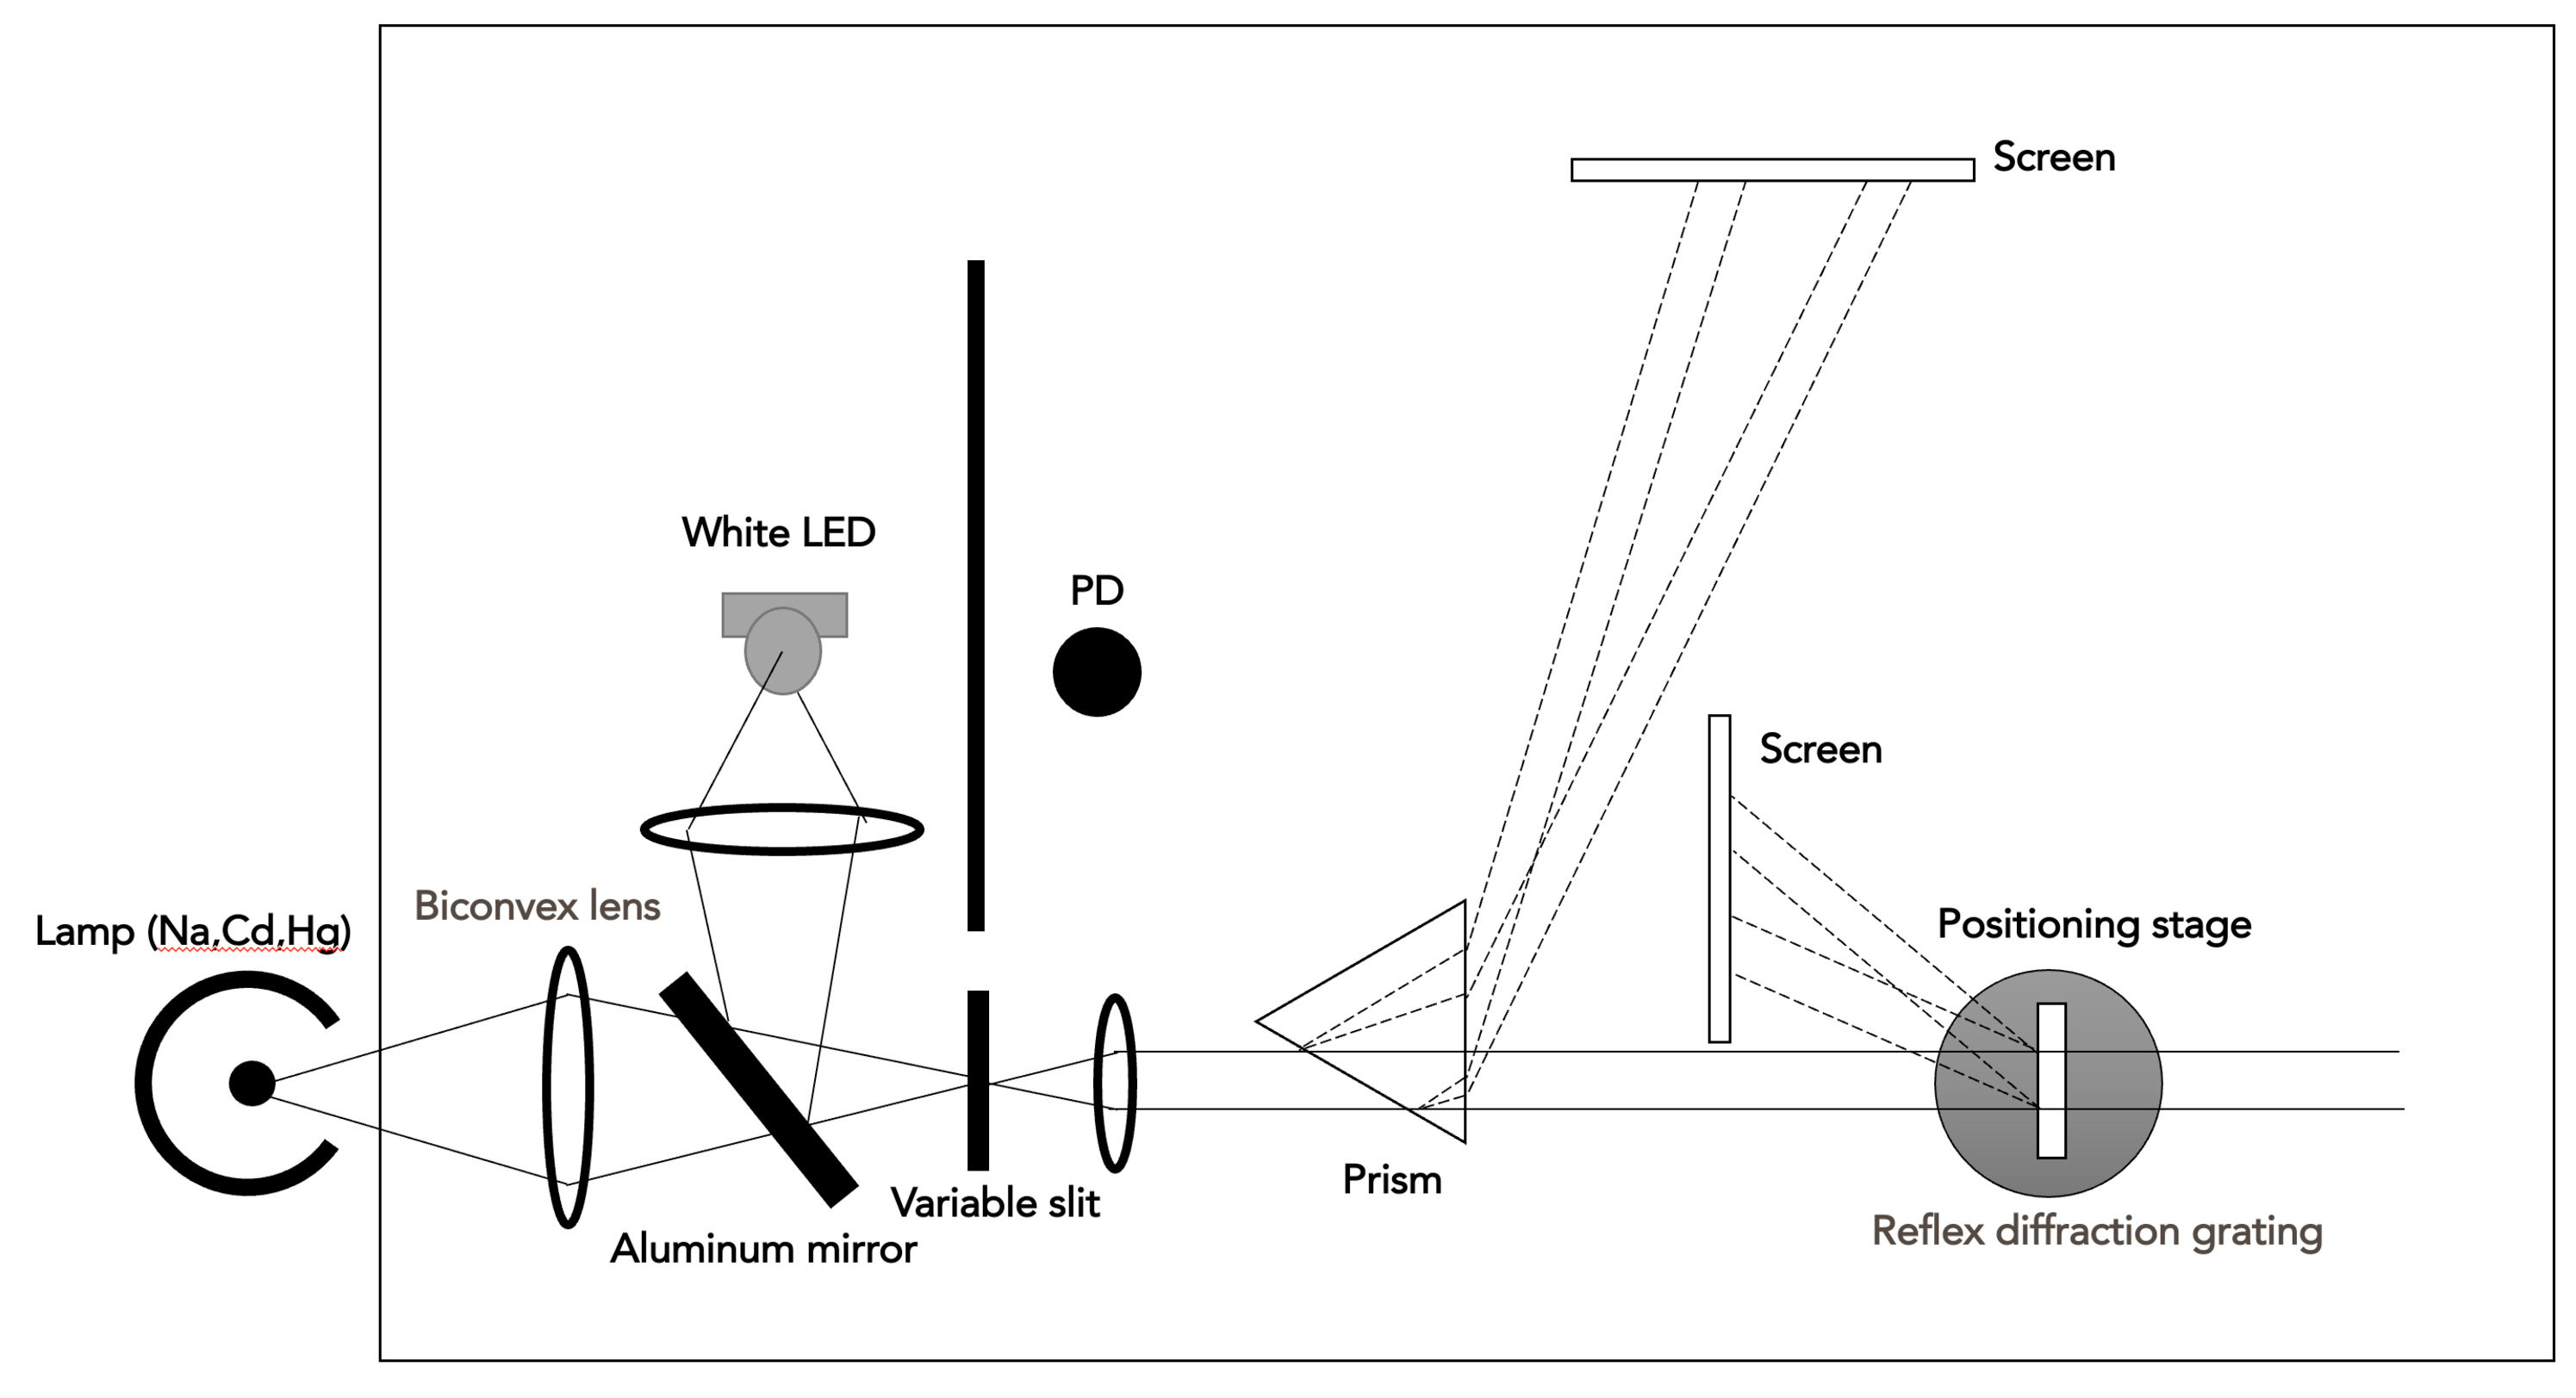
\includegraphics[width=0.8\textwidth]{figs/kougakukei.pdf}
  \caption{測定機器配置図}
\end{figure}


図4は測定系の全体像である。光源は白色(LED)もしくはNa,Cd,Hgランプを使用し、それぞれの光は両凸レンズによって可変スリットに集光させる。光源の切り替えはアルミミラーで行う。可変スリットを通った光はコリメータレンズによって平面波へ変換する。
光強度は、フォトダイオード(PD)の出力電圧によって測定される。

\begin{multicols}{2}
  
\subsection{反射型回折格子による波長分布の測定}
1-2節で述べたように、反射型回折格子で検出される回析光の条件は(3)式
$$d\{\sin(\theta_r+\phi)+\sin\theta_r\} = m\lambda$$
で与えられる。


なので、光を回析格子に垂直に入射することで$\theta_r = 0$とし、回析した1次光をスクリーンで観測することで、その光の波長$\lambda$は
\begin{equation}
  \lambda = d\sin\phi
\end{equation}
で求められる。
$\phi$は入射光と回析光のなす角であるから、図5のように、スクリーンと回析光の距離$L$、スクリーン上の回析光の位置$x$を測定することで、$\tan$の逆関数から$\phi$を求めることができる。


まず、回転ステージに反射型回折格子を設置し、白色LEDの光を回折格子に垂直に入射した。
(0 次光が入射光と重なるようにした)反射型回折格子からの1次の回折光を観測できるようにスクリーンを固定した。回折角により赤〜紫と変化していることが確認できた。
回折格子からスクリーンまでの距離$L$を定規を用いて測定した。
次に光源をNa、Hg、Cdランプの順に変え、各輝線に対する回折光をスクリーン上で確認し、回析光の位置$x
$を計測した。
スクリーン上の回析光の位置$x$は、スクリーンに目盛りをつけて測定した。
\\

\begin{figurehere}
  \centering
  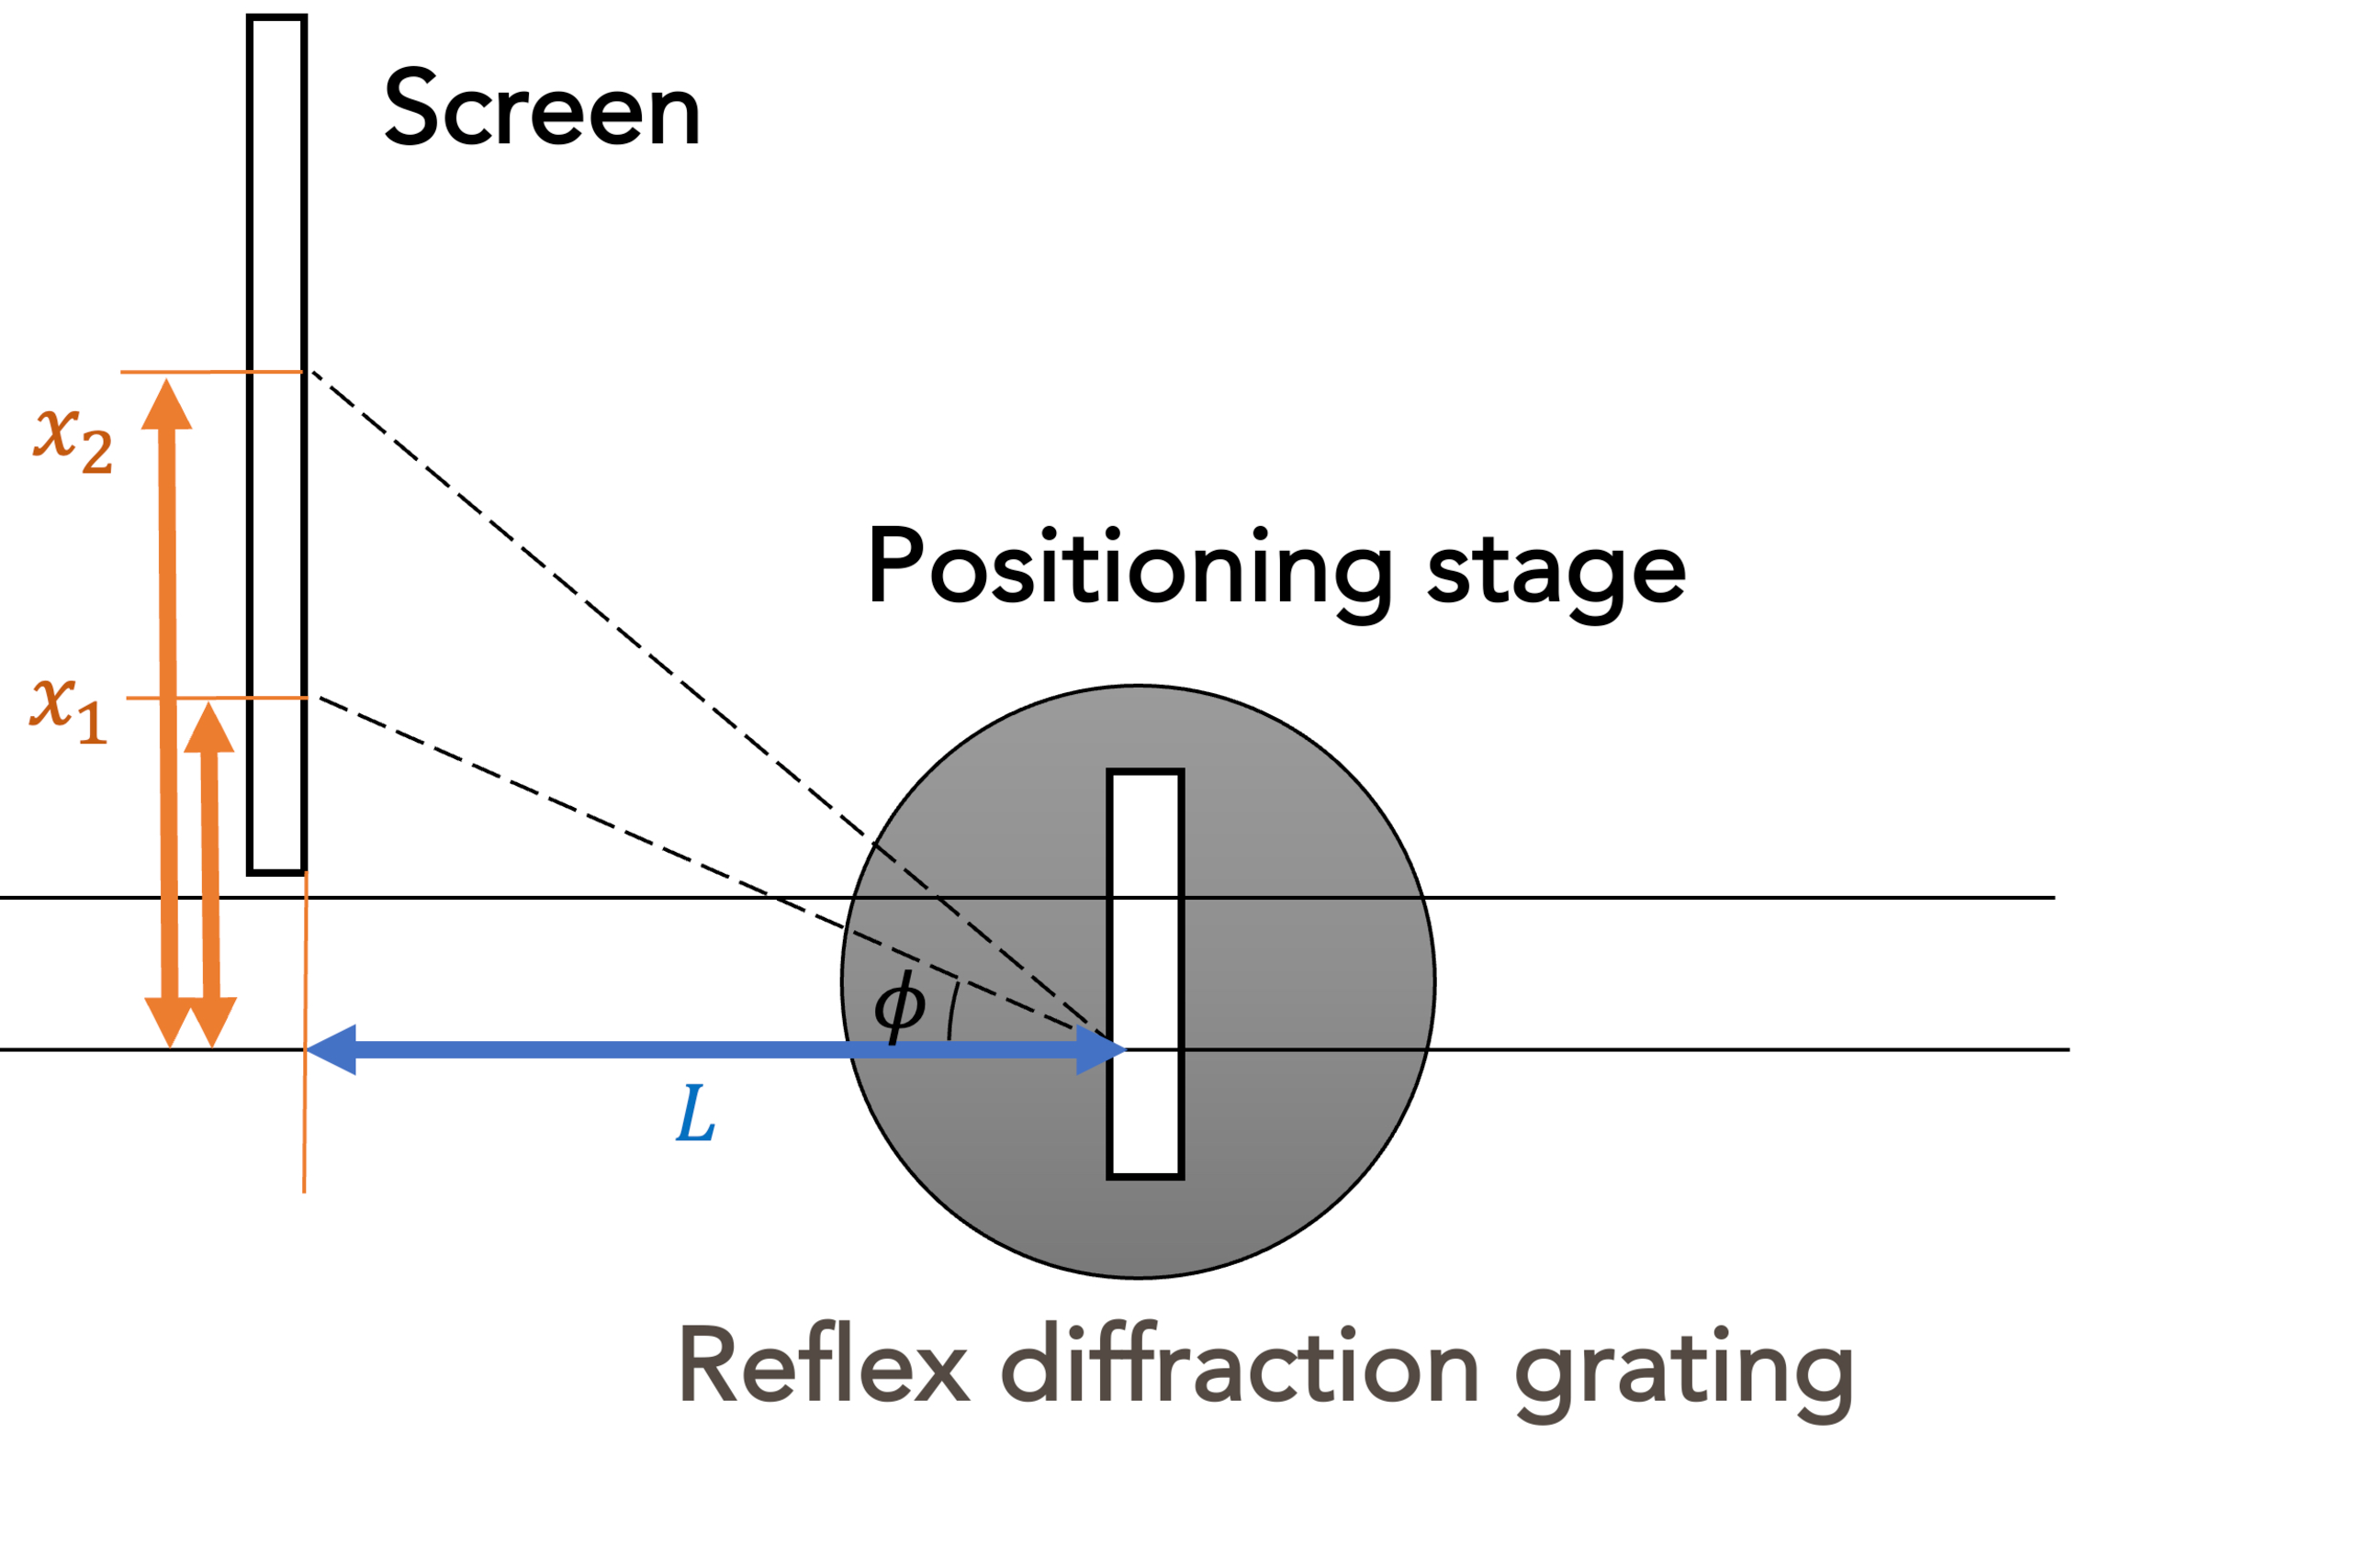
\includegraphics[width=0.5\textwidth]{figs/sample1.pdf}
  \caption{反射型回折格子の回折角測定}
  \label{fig:fig1}
\end{figurehere}

\subsection{屈折率の波長依存性の測定}
各波長$\lambda$における最小偏角$\delta_{min}$を求め、(2)式より各波長に対する屈折率を計算した。
$\delta_{min}$はスクリーンとの距離、輝線の位置を測定することで求めた。
\\

\begin{figurehere}
  \centering
  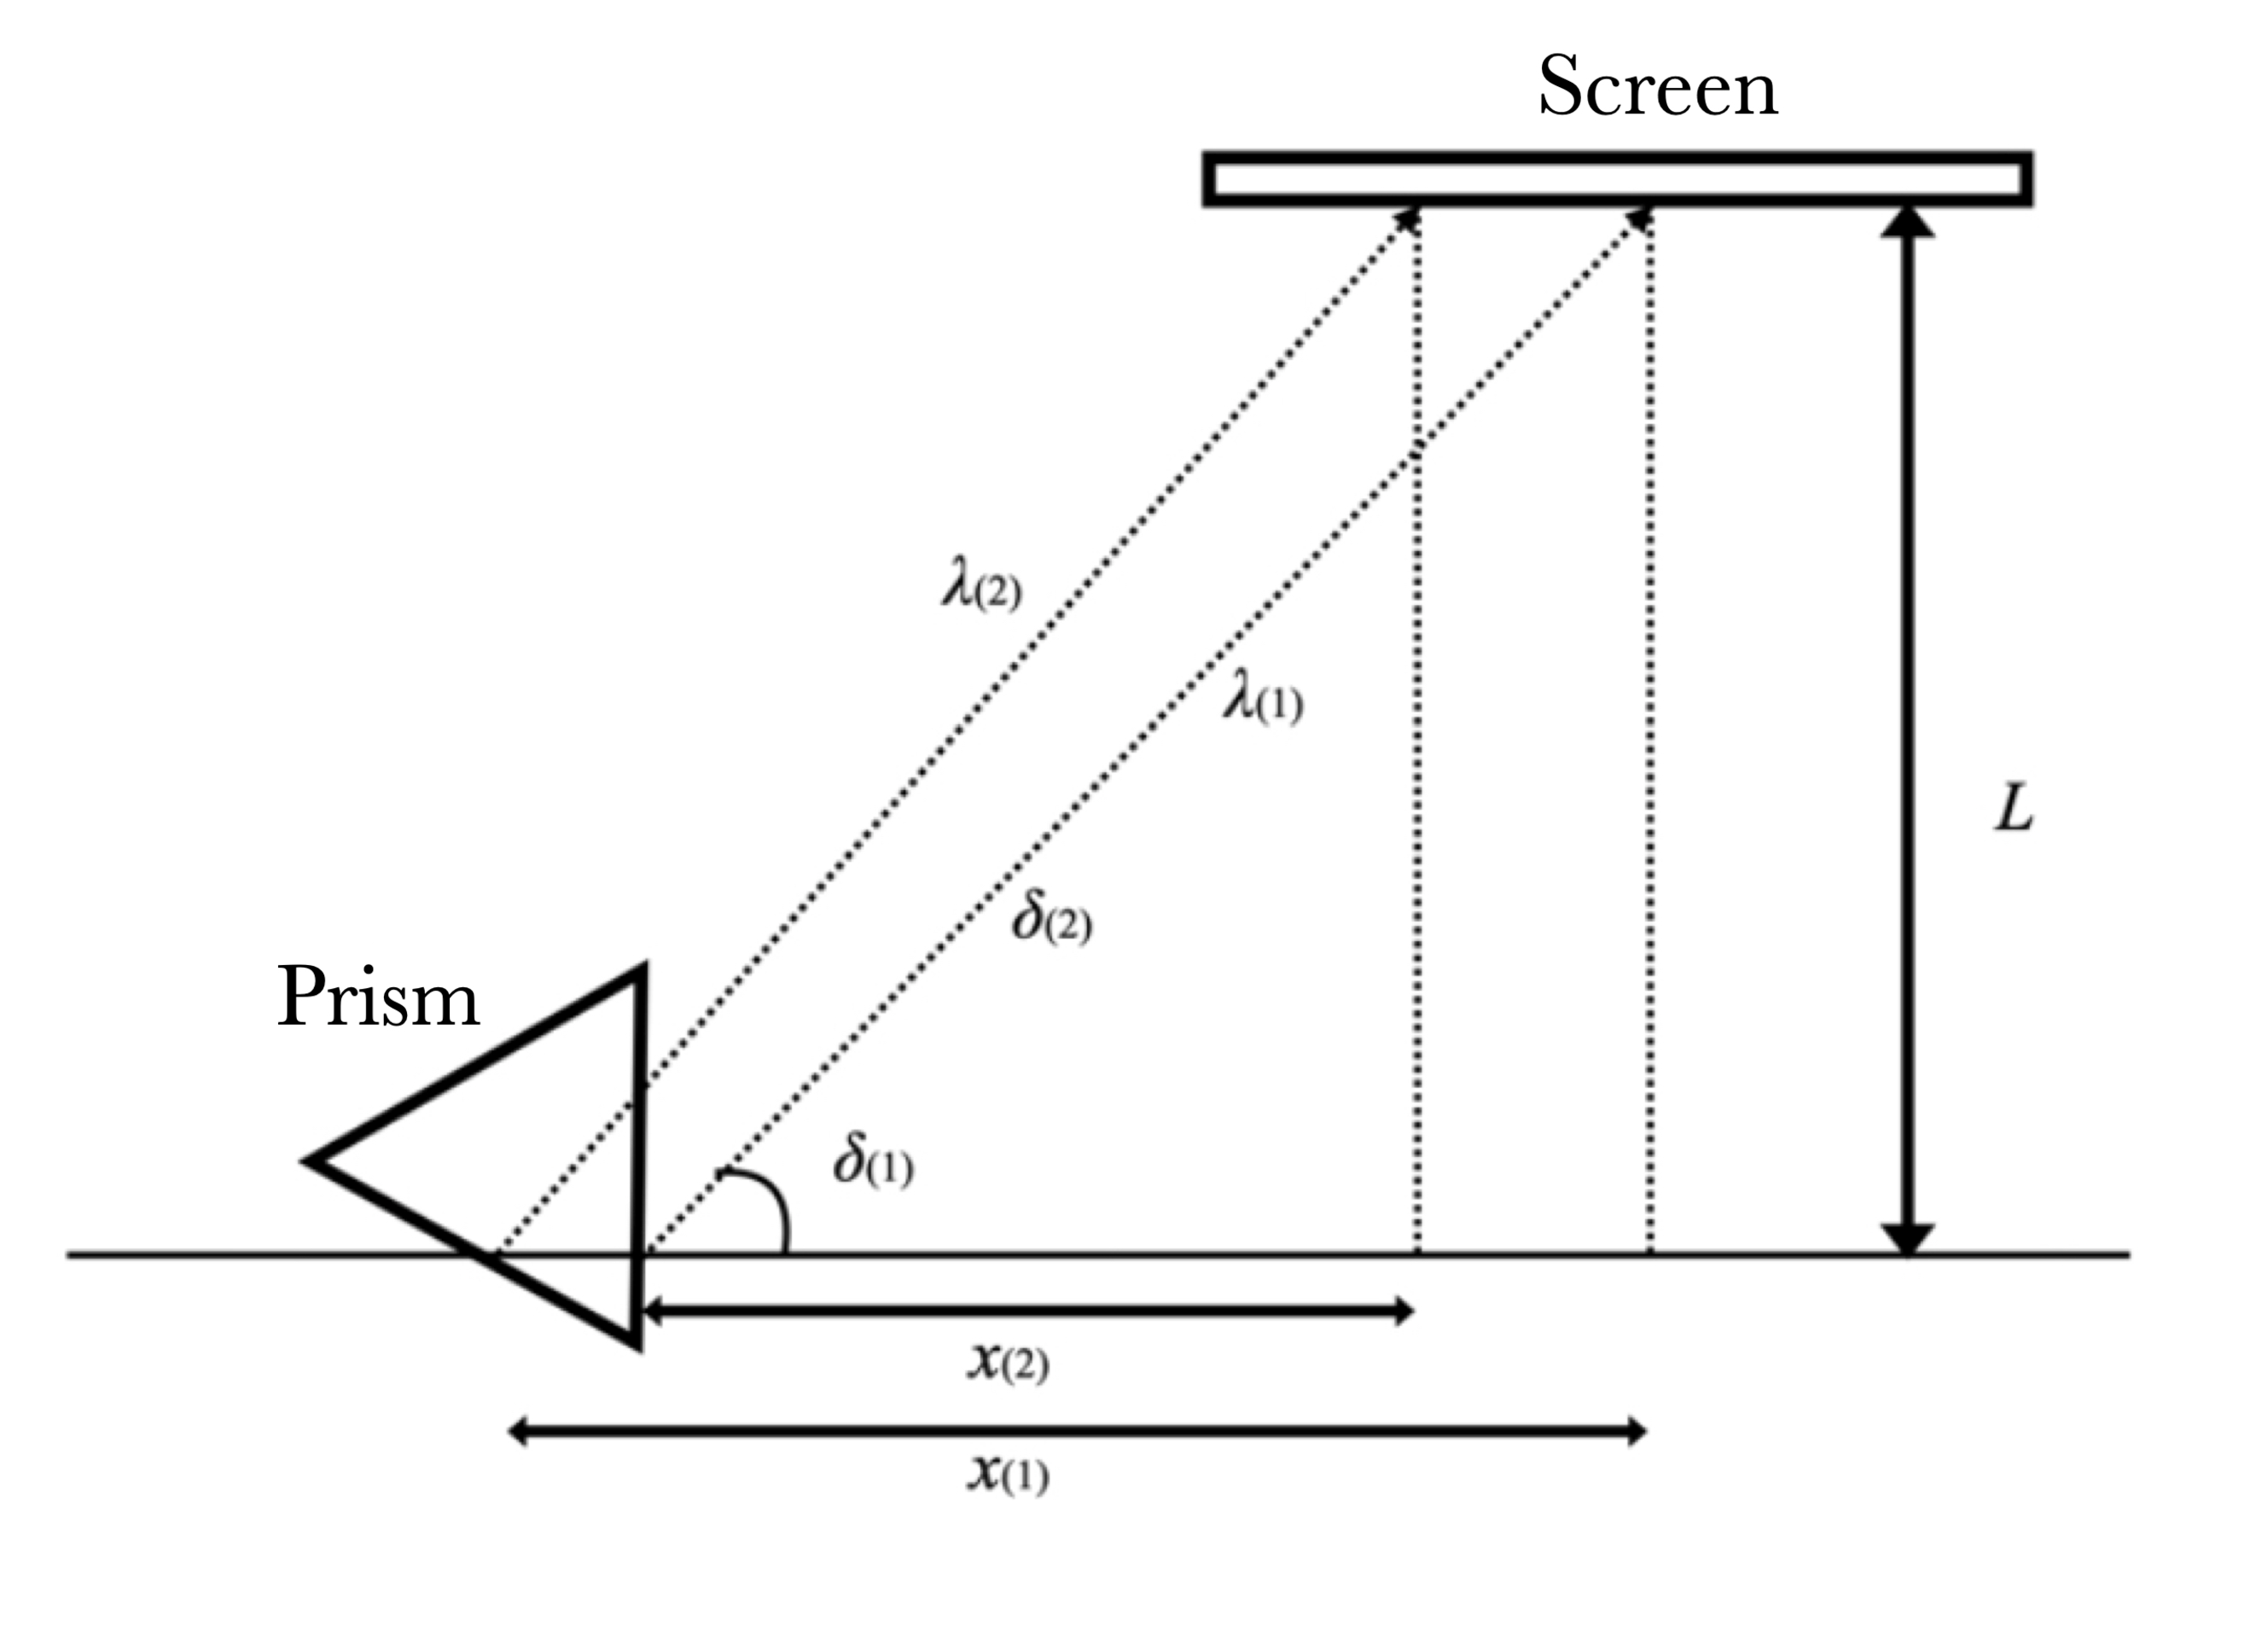
\includegraphics[width=0.5\textwidth]{figs/prism.pdf}
  \caption{プリズムによる偏角の測定}
  \label{fig:fig1}
\end{figurehere}
まず、図4のように、回析格子の間にプリズムを置き、Cdランプの光を当てた。
可変スリットの幅は200\textmu mとした。プリズムを通り分光された光をスクリーン上で観察できるように、スクリーンを固定し、プリズムからスクリーンの長さ$L$を測った。
スクリーン上にCdランプの輝線が縦線として映し出されることを確認したら、各輝線$\lambda_{(1)}$、$\lambda_{(2)}$..に対して偏角$\delta_{(1)}$、$\delta_{(2)}$が最小値になるようにプリズムの角度を微調整し、最小偏角の値を図6の$x_1$、$x_2$..の長さを測ることで計算した。
スクリーンの位置を変え、計3回の計測を行なった。

輝線の波長は$\lambda$実験2-1で求めたCdランプの波長を文献値と比較し、一番近い文献値に対する屈折率を計算した。

\subsection{白色LEDのスペクトル測定}

白色LEDのスペクトルを求めるには、白色LEDの$\lambda$-$\theta$特性が必要になるが、その計測は面倒なので、Cdランプで波長校正曲線を求めることで、白色光LEDの放射スペクトルを得ることができる。
正確には、(3)式を変形したものが校正曲線であるが、フィッテングは2次間数で行なった。

初めに、回転ステージに反射型回折格子を固定し、白色光が垂直に入射するようにした。平凸レンズは、回折格子側を凸とした。
増幅フォトダイオードはスリット面を回折格子側に向け、その前面は回折格子に対して垂直に向くようにした。ある特定の回折角への光のみが集光レンズを通ってスリット中心に焦点が結ばれており、スリットを抜けて検出素子へ到達する。
それとは異なる方向への回折光は、レンズを通ったのち、スリットの壁にぶつかるため検出器までは到達しない。

まず、波長校正曲線の測定実験を行なった。
反射型回折格子にCdランプの光を垂直に入射した。1次の回折光を検出できるようにした。出力電圧が最も高くなる時の回転ステージの位置と出力電圧この測定を記録した。

次に、白色LEDのスペクトル測定を行なった。
この実験は波長校正曲線を用いて行うため、回折格子を抜き取るなど設定が変わる行為を行ってはならない。
白色LEDの光を反射型回折格子に入射した後、回転ステージを連続的に回転させながら、1次回折光の光強度を測定した。
この際、波長校正曲線を参考にして波長範囲300〜800nmあたりで測定した。

\section{Results}

\subsection{反射型回折格子による波長分布の測定}
Naランプでは、橙の光線が観測された。Hgランプでは、青、緑、赤の3つの光線が観測された。
Cdランプでは、紫、青、緑、赤の4つの光線が観測された。
各輝線に対する回析光の位置$x$と、スクリーンまでの距離$L$を測定し、(4)式を用いて波長を計算した結果、表1のようになった。
文献値から比較しても、実験値は文献値に近い値を取っていることがわかる。
% Table generated by Excel2LaTeX from sheet 'Sheet1'
\begin{table*}[htbp]  
  \centering
  \caption{$L$、$x$の測定結果と各輝線の波長($L$:スクリーンまでの距離、$x$:輝線までの距離)}
    \begin{tabular}{lrrrrrrrrrr}
    \toprule
    Type of Lamp & \multicolumn{1}{l}{sodium (Na)} &       & \multicolumn{3}{l}{mercury(Hg)} &       & \multicolumn{4}{l}{cadmium (Cd)} \\
    \midrule
    Observed Color & \multicolumn{1}{l}{Orange} &       & \multicolumn{1}{l}{Blue} & \multicolumn{1}{l}{Green} & \multicolumn{1}{l}{Red} &       & \multicolumn{1}{l}{Purple} & \multicolumn{1}{l}{Blue} & \multicolumn{1}{l}{Green} & \multicolumn{1}{l}{Red} \\
    $L$ [cm] & 15.1  &       & 17.7  & 17.7  & 17.7  &       & 11.4  & 11.4  & 11.4  & 11.4 \\
    $x$ [cm] & 15.2  &       & 10.2  & 14.9  & 16.8  &       & 8.2   & 8.4   & 9.5   & 13.4 \\
    Arctan$(x/L)$ [rad] & 0.789 &       & 0.523 & 0.700 & 0.759 &       & 0.594 & 0.635 & 0.646 & 0.866 \\
    $\lambda$ [nm] & 591   &       & 416   & 537   & 574   &       & 466   & 494   & 502   & 635 \\
    Literature Value [nm] & 589.592 &       & 435.835 & 546.074 & 576.959 &       & 467.815 & 479.992 & 508.582 & 643.847 \\
    \bottomrule
    \end{tabular}%
  \label{tab:addlabel}%
\end{table*}%

\subsection{屈折率の波長依存性の測定}
Cdランプで観測した、緑、青、紫の4つの光線に対して、偏角が最小となる位置を測定した。
赤、緑、青、紫の4つの光線の位置$x_1$、$x_2$、$x_3$、$x_4$を表2に示す。
$L$は、反射型回折格子の中心からスクリーンまでの距離であり、3回位置を変えて測定した。

% Table generated by Excel2LaTeX from sheet '______'
\begin{tablehere}
  \centering
  \caption{Cdランプにおけるプリズムの最小偏角の位置の測定}
    \begin{tabular}{llllll}
    \toprule
          & $L$[cm]     & $x_1$[cm] & $x_2$[cm]& $x_3$[cm]& $x_4$[cm]\\
    \midrule
    1st & 18.2  & 16.7  & 16.4  & 16.1  & 15.4 \\
    2nd & 25.3  & 21.5  & 21.0    & 20.7  & 20.6 \\
    3rd & 10    & 9.3   & 8.5   & 8.3   & 8.1 \\
    \bottomrule
    \end{tabular}%
  \label{tab:addlabel}%
\end{tablehere}%\\
\\

$L$,$x$から最小偏角$\theta$を求め、(2)式から屈折率$n$を求めた。正三角形のプリズムであることより、頂角$\alpha$= 60とした。

表3は、求まった屈折率$n$の平均値である。

% Table generated by Excel2LaTeX from sheet '______'
\begin{tablehere}
  \centering
  \caption{Cdランプにおけるプリズムの屈折率の計算結果}
    \centering
    \begin{tabular}{lrrrr}
    \toprule
    Color & \multicolumn{1}{l}{Red} & \multicolumn{1}{l}{Green} & \multicolumn{1}{l}{Blue} & \multicolumn{1}{l}{Purple} \\
    \midrule
    $n$ & 1.618 & 1.631 & 1.636 & 1.643 \\
    \bottomrule
    \end{tabular}%
  \label{tab:addlabel}%
\end{tablehere}%
\\

長波長になるにつれて、屈折率が大きくなることがわかる。

波長と屈折率の関係性を詳しく見るために、横軸波長$\lambda$、縦軸屈折率$n$としてプロットした。
$\lambda$は、実験2-1で求めた一番近い値の文献値を用いた。

\begin{figurehere}
 \centering
 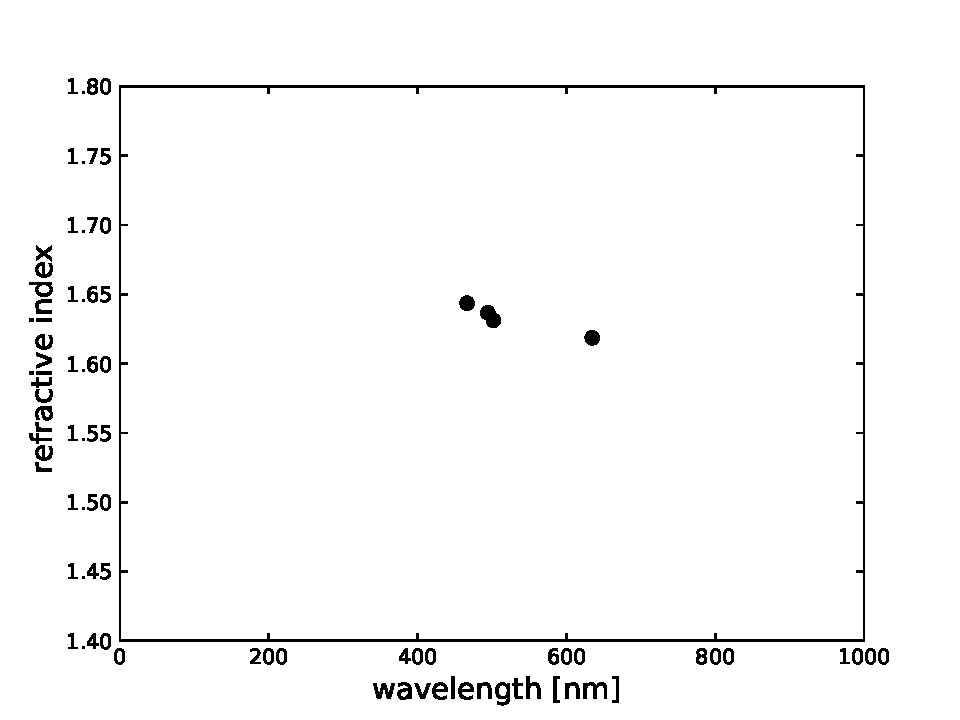
\includegraphics[width=0.5\textwidth]{figs/n-lambda_plot.pdf} 
 \caption{波長と屈折率の関係}
\end{figurehere}

図1と同じスケールでプロットすると、ほぼ直線的に並んだ。

波長領域を可視光に限った為、ほぼ直線的に並んだが、これより短波長側では、屈折率の変化率が大きくなることが予想される。

 
\subsection{白色LEDのスペクトル測定}
初めに、Cdランプの波長校正曲線の測定を行った。
表4は、スリット幅を200\textmu mにした時のCdランプの角度、色毎の電圧の測定結果である。

% Table generated by Excel2LaTeX from sheet '____'
\begin{tablehere}
  \centering
  \caption{スリット幅200\textmu mでの最大電圧近辺の回転角と出力電圧の測定}
    \begin{tabular}{lllll}
    \toprule
    Color & Purple & Blue  & Green & Red \\
    \midrule
    Wavelength[nm] & 466   & 494   & 502   & 635 \\
    Angle [$°$] & 220   & 219   & 219   & 213 \\
    Votage{mVDC} & 8     & 15    & 24    & 21 \\
    \bottomrule
    \end{tabular}%
  \label{tab:addlabel}%
\end{tablehere}%
\\

この結果を元に、電圧と波長の関係をプロットすると、図8のようになった。

\begin{figurehere}
 \centering
 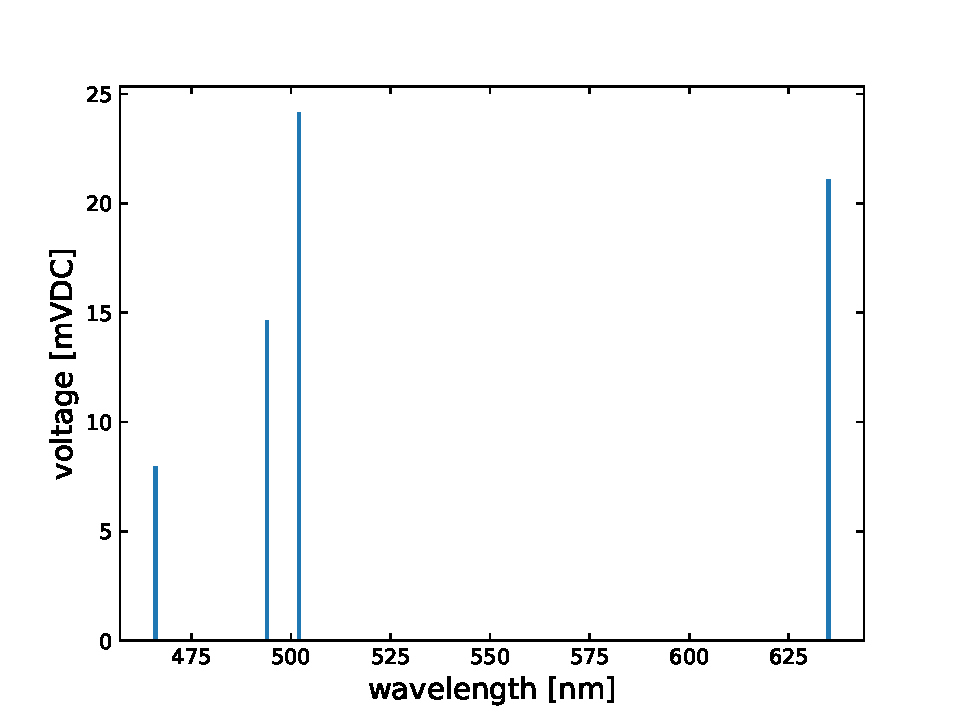
\includegraphics[width=0.5\textwidth]{figs/output.pdf} 
 \caption{Cdランプの波長際の出力電圧}
\end{figurehere}
出力電圧は、緑色の波長が最大であることがわかる。

白色LEDのスペクトル分布を測定するために、波長校正曲線を求めた。
波長$\lambda$の文献値を元に、横軸$\theta$、縦軸$\lambda$としてプロットすると、図9のようになった。

二次関数としてフィッティングを行い、波長校正曲線を求めた結果、波長校正曲線の式は
\begin{equation}
  \lambda = - 0.43\theta^2 + 159.80\theta - 13996.71
\end{equation}
となった。

\begin{figurehere}
  \centering
  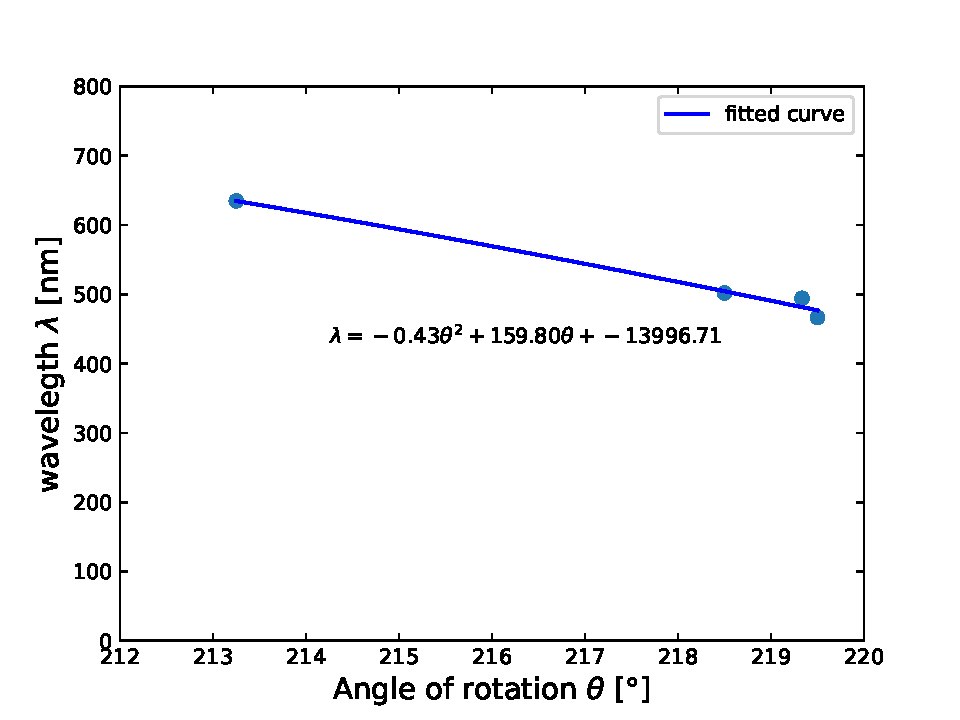
\includegraphics[width=0.5\textwidth]{figs/fitted_curve.pdf}
  \caption{波長校正曲線}
\end{figurehere}

次に、光源を白色LEDに変え、スリット幅を200\textmu mにした時の白色LEDの角度、角度毎の電圧を測定した。

波長校正曲線(5)式を用いて、回転角度を波長に変換し、波長に対する電圧の関係をプロットした。
図10は、横軸波長、縦軸電圧としてプロットした結果である。

\begin{figurehere}
  \centering
  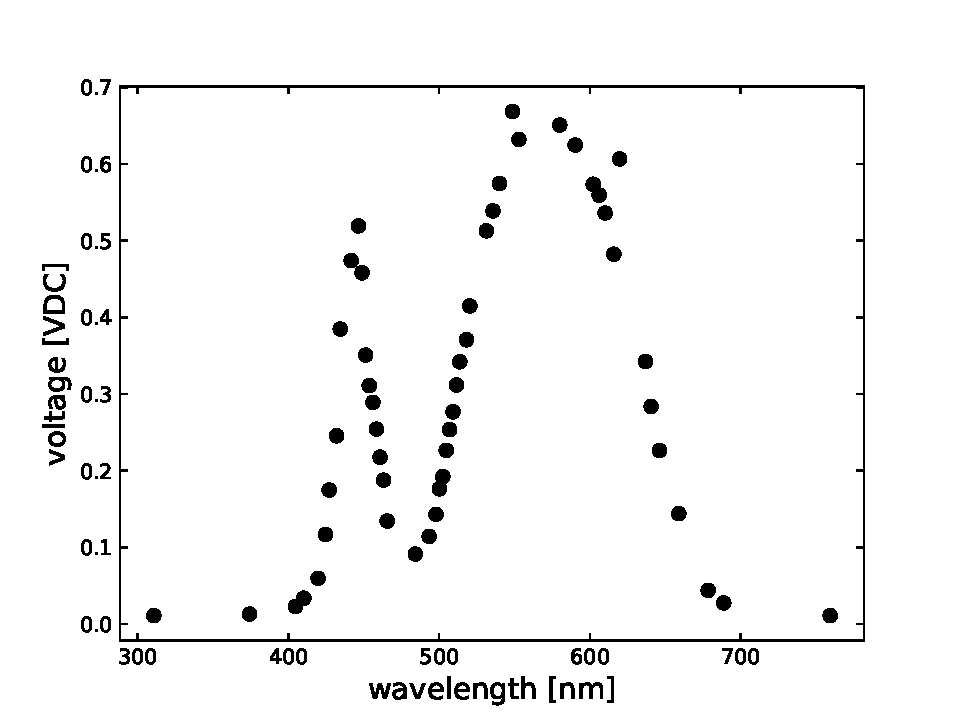
\includegraphics[width=0.5\textwidth]{figs/scatter_plot.pdf}
  \caption{白色LEDのスペクトル分布}
\end{figurehere}

図10より、白色LEDから出ている光は2回極値を取っていることが分かる。
一つ目は、波長460nm付近で鋭いピークを持ち、二つ目は、波長560nm付近で緩やかなピークを持つことが確認できる。
これは、白色LEDが、青色LEDと黄色LEDを混ぜたものであることを示している。

図3と比較すると、青色光のピークは小さくなっているが、極値を取っている波長の位置は、ほぼ同じであることが分かる。
従って、波長校正は正しく行われていると考えられる。


550nm、610nm付近で、はずれ値が見られるが、これは、スリット幅が200\textmu mと狭く、光の強度が弱かったため、他の光源の影響を受けたものだと考えられる。
\section{Discussion}
\subsection{スペクトル分解能についての議論}
表1を見ると、測定値と文献値に大きなズレはなかったが、これ以上の精度で測定することはできないだろか。測定時を振り返ると、スクリーンに映るスペクトルの幅は大きく、光線の位置を正確に測ることが難しかった。
このスペクトルの幅を狭くすることができれば、より正確な波長を測定することができるだろう。

スペクトル分解を行う際は、回折格子の溝と光が干渉する際に、波面が平坦であることが重要である。スリット幅が広い場合は、光が広がり波面が不均一になるため、干渉縞がぼやけてしまう。一方、スリット幅が狭い場合は、光が集まり、波面が平坦であるため、干渉縞が鮮明に現れる。
従って、理論上は、スリット幅を狭くすることで、スペクトルの幅を狭くすることができると考えられる。

図11はCdランプのスペクトルのピーク時である500nm付近で、スリット幅を変えた時のスペクトルを観測した結果である。
スリット幅200\textmu m時のスペクトルは青、スリット幅1000\textmu m時のスペクトルは赤でプロットしている。

\begin{figurehere}
 \centering
 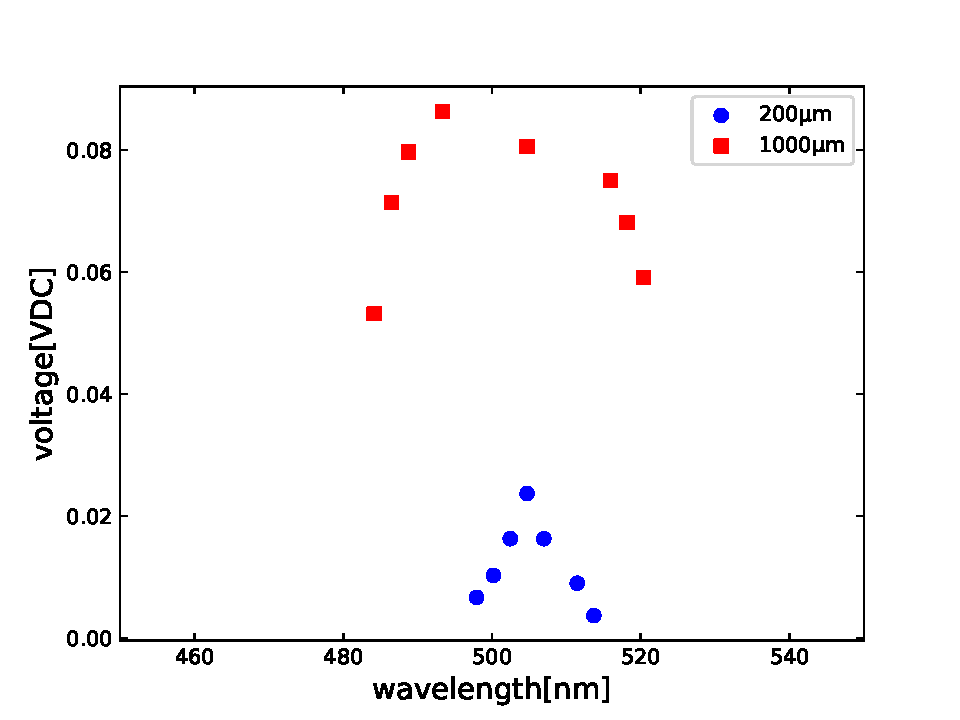
\includegraphics[width=0.5\textwidth]{figs/slit_comparison.pdf} 
 \caption{Cdランプのスリット幅1000\textmu m、200\textmu mの時のスペクトル}
\end{figurehere}

スリット幅200\textmu mの時のスペクトルは、波長が500nm付近でピークを取っていることが分かるが、スリット幅1000\textmu mの時のスペクトルは、スペクトルの幅が広く、ピークがぼやけていることが分かる。

従って、スリット幅を200\textmu mよりも狭くすることができれば、より正確な波長を測定することができると考えられる。
しかし、200\textmu mよりも狭くすると、光の強度が弱くなり、他の光源の影響を大きく受けるため、スペクトルのピークを測定することが難しくなる。
そう考えると、今回の実験環境ではスリット幅200\textmu mが最適であると考えられる。

\subsection{屈折率の波長依存性}
3-2の結果から分かるように、物質の屈折率は、波長によって変化する。
この現象は、分散と呼ばれる。では、この分散がどのように起こるかを簡単なモデルで説明しよう。

屈折率は注目する新空中の光の速さ$c$と、物質中の光の速さ$v$の比である。光の速さは、誘電率$\varepsilon$と透磁率$\mu$を用いて、$c = \frac{1}{\sqrt{\varepsilon \mu}}$と表されるので、屈折率$n$は
\begin{equation}
  n = \frac{c}{v} = \sqrt{\frac{\varepsilon \mu}{\varepsilon_0 \mu_0}}
\end{equation}
と表される。ここで、$\varepsilon_0$は真空の誘電率、$\mu_0$は真空の透磁率である。
誘電体では、$\mu\approx\mu_0$と置けるので、結局$\varepsilon$と波長の関係を求めれば屈折率の分散の様子がわかる。
電気双極子放射の原理より、光の伝播の様子は分極の振動によって説明できる。

今、原子を構成する電子に角振動数$\omega$をもつ電場
\begin{equation}
  \bm{E(t)} = \bm{E}_0 \exp{i\omega t}
\end{equation}
 が作用したとする。電子の位置を$\bm{x(t)}$、質量を$m$とすると、電子に関する運動方程式は
\begin{equation}
  m\frac{d^2\bm{x(t)}}{dt^2} = -m\omega_0^2\bm{x(t)} + e\bm{E(t)}
\end{equation}
と表される。ここで、$\omega_0$は電子の固有振動数、$e$は電子の電荷である。この式は、振り子に強制振動を与えたような場合を表しており、解は容易に求まる。
計算の結果、外部電場による電子の変位は
\begin{equation}
  \bm{x(t)} = \frac{e}{m(\omega_0^2 - \omega^2)}\bm{E(t)}
\end{equation}
と求まる。

分極$\bm{P}$は単位体積中の電気双極子の数$(N)$で定義できるので、
\begin{align}
  \begin{split}
  \bm{P} &= N\bm{x(t)} \\
         &= \frac{Ne^2}{m(\omega_0^2 - \omega^2)}\bm{E(t)}
  \end{split}
\end{align}
と表される。一方、誘電体の誘電率$\varepsilon$と分極$\bm{P}$の間には、
\begin{equation}
  \varepsilon\bm{E} = \varepsilon_0\bm{E} + \bm{P}
\end{equation}
という関係があるので、誘電率$\varepsilon$は
\begin{align}
  \begin{split}
  \varepsilon &= \varepsilon_0 + \frac{\bm{P}}{\bm{E}} \\
              &= \varepsilon_0 + \frac{Ne^2}{m(\omega_0^2 - \omega^2)}
  \end{split}
\end{align}
となる。屈折率の定義から
\begin{equation}
  n^2 = 1 + \frac{Ne^2}{\varepsilon_0 m}\bigg(\frac{1}{\omega_0^2 - \omega^2}\bigg)
\end{equation}
が求まる。これが角振動数$\omega$の光に対する屈折率を表す式であり、分散式と呼ばれる。
\clearpage
この分散式は密度が小さいガスに対して有効であるが、密度の大きい液体や個体に対しては、分子間の相互作用を考慮する必要がある。
詳しい計算によると、個体等に対しては
\begin{equation}
  \frac{n^2-1}{n^2+2} = \frac{Ne^2}{3\varepsilon_0 m}\bigg(\frac{1}{\omega_0^2 - \omega^2}\bigg)
\end{equation}
の式が利用される。
いずれにせよ、屈折率が入射光の角振動数、すなわち波長に依存することがわかる。

式、(15)から明らかなように、$\omega < \omega_0$の領域、すなわち角振動数が$\omega_0$より小さい領域(波長が長い領域)では、$\omega$が増す(波長が短くなる)につれて屈折率は屈折率も大きくなることがわかる(正常分散)。
分散式からは、$\omega_0 = \omega$(共鳴あるいは共振)付近で屈折率が無限大に発散してしまうが、実際には電子に抵抗力が作用し有限の値となる。
共鳴条件は可視光領域以外の波長域でもいくつか見られ、$\omega$の増加に伴い屈折率が減少する領域もある(異常分散)。

\section{Conclusion}
実験1では、波長分布が与えられたNa,Hg,Cdランプの光をスリットに通し、反射型回折格子に反射させ、分散した光をスクリーンで観測することで、スペクトル分解を行った。
  Cdランプについてはスリット幅が1000\textmu mの時と、200\textmu mの時でスペクトルを観測した。その結果、スリット幅を狭めた方が、スペクトル分解能を向上させることがわかった。

  実験2では、ガラス製三角プリズムにCdランプの光を入射させ、最小偏角を測定することで屈折率を求めた。波長は実験1で求めた値を用いて、波長に対する屈折率の波長依存性を調べた。その結果、屈折率は波長が短くなるにつれて大きくなることが確認できた。
  
  実験3では、白色LEDのスペクトル分布を調べた。白色LEDのスペクトルについては、波長450nmの鋭いピークと、波長580nmを中心とするブロードなピークで構成されていることを確認した。
  450nmは青、580nmは黄色に相当する波長であることから、今回測定した白色LEDは、青色と黄色の発光体を組み合わせて擬似的に白色に見せているものと結論した。

\begin{thebibliography}{文献数}
\bibitem{ID} 青木貞雄,『光学入門』(共立出版)
\bibitem{ID2} 石黒浩三,『光学』(裳華房) 
\bibitem{ID3} 尾中龍猛,『光と個体』


\end{thebibliography}
\end{multicols}
\clearpage
\begin{center}
\section*{Appendix}
\end{center}
\subsection*{プリズムと最小偏角}

ここでは、ある波長に対する物質の屈折率をプリズムの屈折角を利用して求める方法を紹介する。
今、図12のように空気中に置かれた頂角$\alpha$の三角柱プリズム(屈折率$n$)を考える。
\begin{figure}[H]
  \centering
  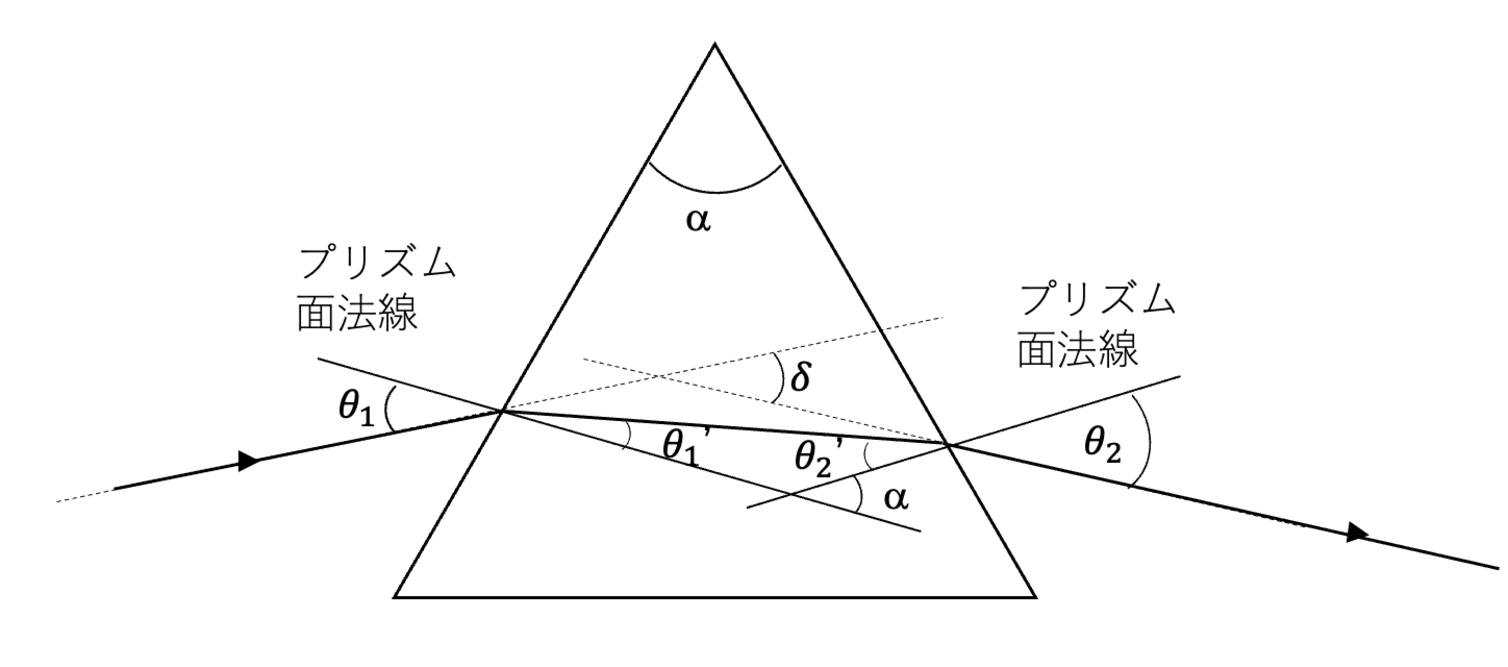
\includegraphics[width=0.5\textwidth]{figs/prism_figure.pdf}
\end{figure}
光は平面に平行に左側から入射し、2回の屈折を経て右側に出射する。入光光線と出射光線のなす角(偏角)を$\delta$とすると
\begin{equation}
  \delta = (\theta_1 - \theta_1') + (\theta_2 - \theta_2')
\end{equation}
である。$\delta$の値は入射光を変えると変化する。光線の逆進性を考えると、$\theta_1'=\theta_2'$のとき、入射光線と出射光線が対象になり、$\delta$の値は極小値をとる。この時の偏角$\delta_{min}$を最小偏角と呼ぶ。
入射角$\theta_1$の変化に対して$\delta$が極値を取る条件は、
\begin{equation}
  \frac{d\delta}{d\theta_1} = 0 = 1 + \frac{d\delta_2}{d\theta_1}
\end{equation}
である。次に$d\aleph=0$より
\begin{equation}
  d\theta_1' + d\theta_2' = 0
\end{equation}
入射点および出射点におけるスネルの法則より
\begin{align}
  \begin{split}
  \sin\theta_1 = n\sin\theta_1' \\
  n\sin\theta_2' = \sin\theta_2
  \end{split}
\end{align}
それぞれの両辺を微分すると
\begin{align}
  \begin{split}
  \cos\theta_1 d\theta_1 = n\cos\theta_1'd\theta_1' \\
  n\cos\theta_2'd\theta_2' = \cos\theta_2 d\theta_2
  \end{split}
\end{align}
式(17), (18), (19)を整理すると
\begin{equation}
  \frac{\cos{\theta_1}}{\cos{\theta_2}} = \frac{\cos{\theta_1'}}{\cos{\theta_2'}}
\end{equation}
となる。両辺を2乗して再びスネルの法則を用いると
\begin{equation}
  \frac{1-\sin^2{\theta_1}}{1-\sin^2{\theta_2}} = \frac{n^2-\sin^2{\theta_1}}{n^2-\sin^2{\theta_2}}
\end{equation}
となる。上の式を整理すると
\begin{equation}
  (n^2-1)(\sin^2{\theta_1}-\sin^2{\theta_2}) = 0
\end{equation}
となり、$n\ne0$なので、$\sin{\theta_1}=\sin{\theta_2}$がいえる。この時の$\delta$の値を$\delta_{min}$とすると
\begin{equation}
  \theta_1 = \frac{\delta_{min}+\alpha}{2}
\end{equation}
となり、$\theta_1'=\theta_2'=\alpha/2$となる。結局、屈折率$n$は(2)式
\begin{equation*}
  n =\sin\{(\alpha+\delta_{min})/2\}/\sin(\alpha/2)
\end{equation*}
で与えられる。

\end{document}